\section{Evaluation: User Studies}

To assess Porta's potential efficacy, we had 12 students activate it
while following 3 software tutorials. We then showed the resulting Porta
outputs to the instructors who created those tutorials. We wanted to
investigate two main questions:

\begin{itemize}\itemsep0pt

\item Does Porta help students better reflect on the difficulties they
faced while following tutorials?

\item Does Porta provide useful feedback to instructors about how to
improve their own tutorials in the future?

\end{itemize}


\textbf{Materials}: For this study, we used three web-based
tutorials created by instructors at our university for classes they
teach:

\begin{itemize}\itemsep0pt

\item \textbf{Python}: A primer on basic Python types, control flow, and
functions; created for a data science course (\texttildelow800 words).

\item \textbf{Git}: Intro.\ to the Git version control system and
GitHub; created as part of a MOOC on introducing scientists
to command-line development tools (\texttildelow3,000 words).
% TODO: think about what to cite in order not to violate anonymity

\item \textbf{Web Design}: Intro.\ to HTML, CSS, and JavaScript with
jQuery; created for an HCI course (\texttildelow500 words).

\end{itemize}

Each tutorial was formatted as step-by-step instructions on a single
vertically-scrolling webpage with mini-exercises for students to check
their understanding. The Web Design tutorial also featured embedded
screenshots and mini-videos.

\textbf{Procedure for Student User Study}: We recruited 12
computer science undergraduate students (9 women) from our university
each for a 1-hour user study; each was paid \$10. To find novices, we
limited recruitment to those who had little to no experience with the
subject of the tutorial they saw.
%
%taken only lower-division courses and had 
%
Each participant came to our lab to work through one tutorial on a macOS
machine with both Porta and the necessary software (e.g., text editors,
terminal app, Python, Git) installed:

\begin{enumerate}\itemsep0pt

\item We activated Porta and gave the participant up to 40 minutes to
work through the tutorial in any way they wished.

\item After stopping Porta, we asked the participant to reflect on any
difficulties they faced while following the tutorial and to provide
suggestions for improving the tutorial. Note that this debriefing occurs
\emph{before} they ever see Porta's output.

\item Finally, we showed the participant the output of Porta and let
them freely explore the profile visualization interface. Throughout this
process, we asked them to further reflect on any suggestions they have
for improving the tutorial.

\end{enumerate}


\textbf{Procedure for Instructor User Study}: After
completing the student user study, each of the 3 tutorials now had
profile information collected from 4 students trying to follow them.
%
For this study, we had the instructors who created each tutorial come to
our lab for one hour and inspect Porta's output:

\begin{enumerate}\itemsep0pt

\item We began by showing the instructor their own tutorial and having
them reflect on if they wished to make any changes to it. Note that this
occurs \emph{before} they ever see Porta.

\item We then showed the instructor Porta outputs from each of the 4
student studies, as well as the aggregate visualization of all 4
sessions together. We let them freely explore the interface. We asked
them to think aloud and again reflect on whether they wished to make any
changes to their tutorial.

%\item Finally, we showed them the \emph{aggregate visualization}
%produced by combining the data from all 4 student user study sessions.
%We again had them reflect on what they saw.

\end{enumerate}


\textbf{Study Limitations}:
%
Our findings came from self-reported anecdotes from first-time users. We
have no evidence of longitudinal effects such as whether the instructors
actually made the suggested improvements to their tutorials or whether
future students ended up benefiting from those improvements.

We also opted for a within-subjects study design so that we could
directly compare the nature of each participant's feedback before and
after they saw Porta's output. There may be some ordering effects, but
it is infeasible to flip the order of exposure: i.e., if we first show
someone Porta's output, then they cannot ``un-see" it later in the
session. To get an additional baseline for comparison, we could follow
up with a between-subjects study where we show one group a raw
screencast video recording of the test session instead of Porta's
output. (Note that Porta includes a full screencast recording of the
session, but it is segmented based on events.)

%We tried to simulate an end-to-end user scenario where Porta would be
%used by both the creators and consumers of each tutorial. We could have
%obtained more external validity if tutorial creators had purposely
%sought out Porta to use for running their own user studies instead of
%being recruited for a controlled lab study.



\subsection{Findings from Student User Study}

\tab{tab:consumer-study} summarizes Porta's recordings for the 12
participants in the student user study (P1--P12). Everyone completed
their tutorial within the 40 minutes they were given. Since we did not
formally assess students' understanding of the subjects, it is possible
that they made mistakes while performing the given actions or harbored
some misconceptions; however, we feel that this is a realistic simulation
since students would not be supervised when following these tutorials on
their own.

\tab{tab:consumer-study} also shows the occurrences of events that Porta
recorded during each session. Taken together, these three tutorials elicited all
event types: The Python tutorial involved running shell
commands, the Git tutorial involved ssh-based commands to use Git on
a remote server, and the Web tutorial involved Chrome developer tool
interactions.
%
Although we did not formally measure application run-time speeds,
participants did not report any performance-related problems.

\textbf{Feedback comparison}: \tab{tab:study-feedback} contrasts
the qualitative feedback that participants provided before and after
seeing Porta's output.
%
Before seeing Porta's output, they provided either vague or non-existent
feedback. We gave each one the opportunity to look through their
tutorial again, and 8 out of 12 participants felt like it was good
enough in its current state. For instance, P1 said that the Python
tutorial was ``easy to follow" and P5 said the Git tutorial ``seemed
straightforward." When they did offer critiques, their descriptions were
high-level: e.g., ``language could be more novice friendly" (P8).

In contrast, once participants started exploring Porta's output, they
were able to give much more specific and targeted feedback. Everybody
had at least one concrete suggestion for improvement, even those who
minutes earlier had just said that the tutorial looked fine as-is. The
upper right of \tab{tab:study-feedback} shows one example from each
participant. Aside from being specific, each suggestion was made while
referencing a specific location in the tutorial, so they were precisely
targeted.

For example, both P3 and P4 originally said the tutorial looked fine,
but as they explored Porta's output they zoomed in on occurrences of
errors while running Python commands. They saw that there were error
messages related to them using ``true" and ``false" for booleans instead
of the properly capitalized versions (``True" and ``False") that Python
requires. They suggested for the tutorial creator to add a clarifying
note there to help students who were used to bools in other languages.

In theory, participants could glean this same information from watching
a raw screencast video recording of their sessions, but it would likely
be harder to pinpoint occurrences of key events in a 40-minute-long
video. Porta's visualizations allowed participants to quickly zoom in on
key events such as command invocations and toolchain errors so that they
watched only the video segments centered at those events. \emph{Porta thus
provides a convenient event- and time-based index into the underlying
raw screencast videos that it records.}

\begin{mynote}

\textbf{Summary}: Porta allowed test participants to give more specific
and targeted feedback on how to improve tutorials.

\end{mynote}

\begin{table}%[h]
\small % TODO: will this corrupt everything that comes afterward?
\centering
\begin{tabulary}{\columnwidth}{@{}L@{}C@{}R|@{}C@{}CC|C@{}C@{}C@{}}
& & & \multicolumn{3}{c|}{\# application events} & \multicolumn{3}{c}{\# web browser events} \\
\multicolumn{2}{@{}l@{}}{Participant} \hspace{0.06em} & Time & \hspace{0.3em} Local (errors) & \hspace{0.2em} Remote & Clip & Pages \hspace{0.2em} & Devtools \hspace{0.2em} & Errors \\
\hline
P1  & Py & 38   & 50 (10) & 0 & 0 & 0 & 0 & 0 \\
P2  & Py & 26   & 35 (1)  & 0 & 23 & 0 & 0 & 0 \\
P3  & Py & 26   & 36 (5)  & 0 & 12 & 0 & 0 & 0 \\
P4  & Py & 29   & 30 (3)  & 0 & 18 & 0 & 0 & 0 \\
\hline
P5  & Git & 24  & 0 & 57 & 0 & 0 & 0 & 0 \\
P6  & Git & 28  & 0 & 73 & 0 & 0 & 0 & 0 \\
P7  & Git & 21  & 0 & 52 & 0 & 0 & 0 & 0 \\
P8  & Git & 21  & 0 & 49 & 33 & 0 & 0 & 0 \\
\hline
P9  & Web & 28  & 0 & 0 & 9 & 2 & 0 & 2 \\
P10\hspace{0.5em} & Web & 17  & 0 & 0 & 0 & 2 & 0 & 5 \\
P11 & Web & 21  & 0 & 0 & 8 & 4 & 1 & 3 \\
P12 & Web & 37  & 0 & 0 & 0 & 10 & 1 & 2 \\
\hline

\end{tabulary}

\caption{Summary of Porta events recorded during the 12 student user
study sessions for Python, Git, and Web Design tutorials. Session time
is in minutes. ``Local" events include both shell commands and
compiler/interpreter toolchain (e.g., Python) invocations. ``Clip" is
clipboard copy-and-paste. ``Pages" is opening additional webpages in new
tabs.}

%\vspace{-0.5em} % stent
\label{tab:consumer-study}
\end{table}



\begin{table}
  \label{tab:study-feedback}
  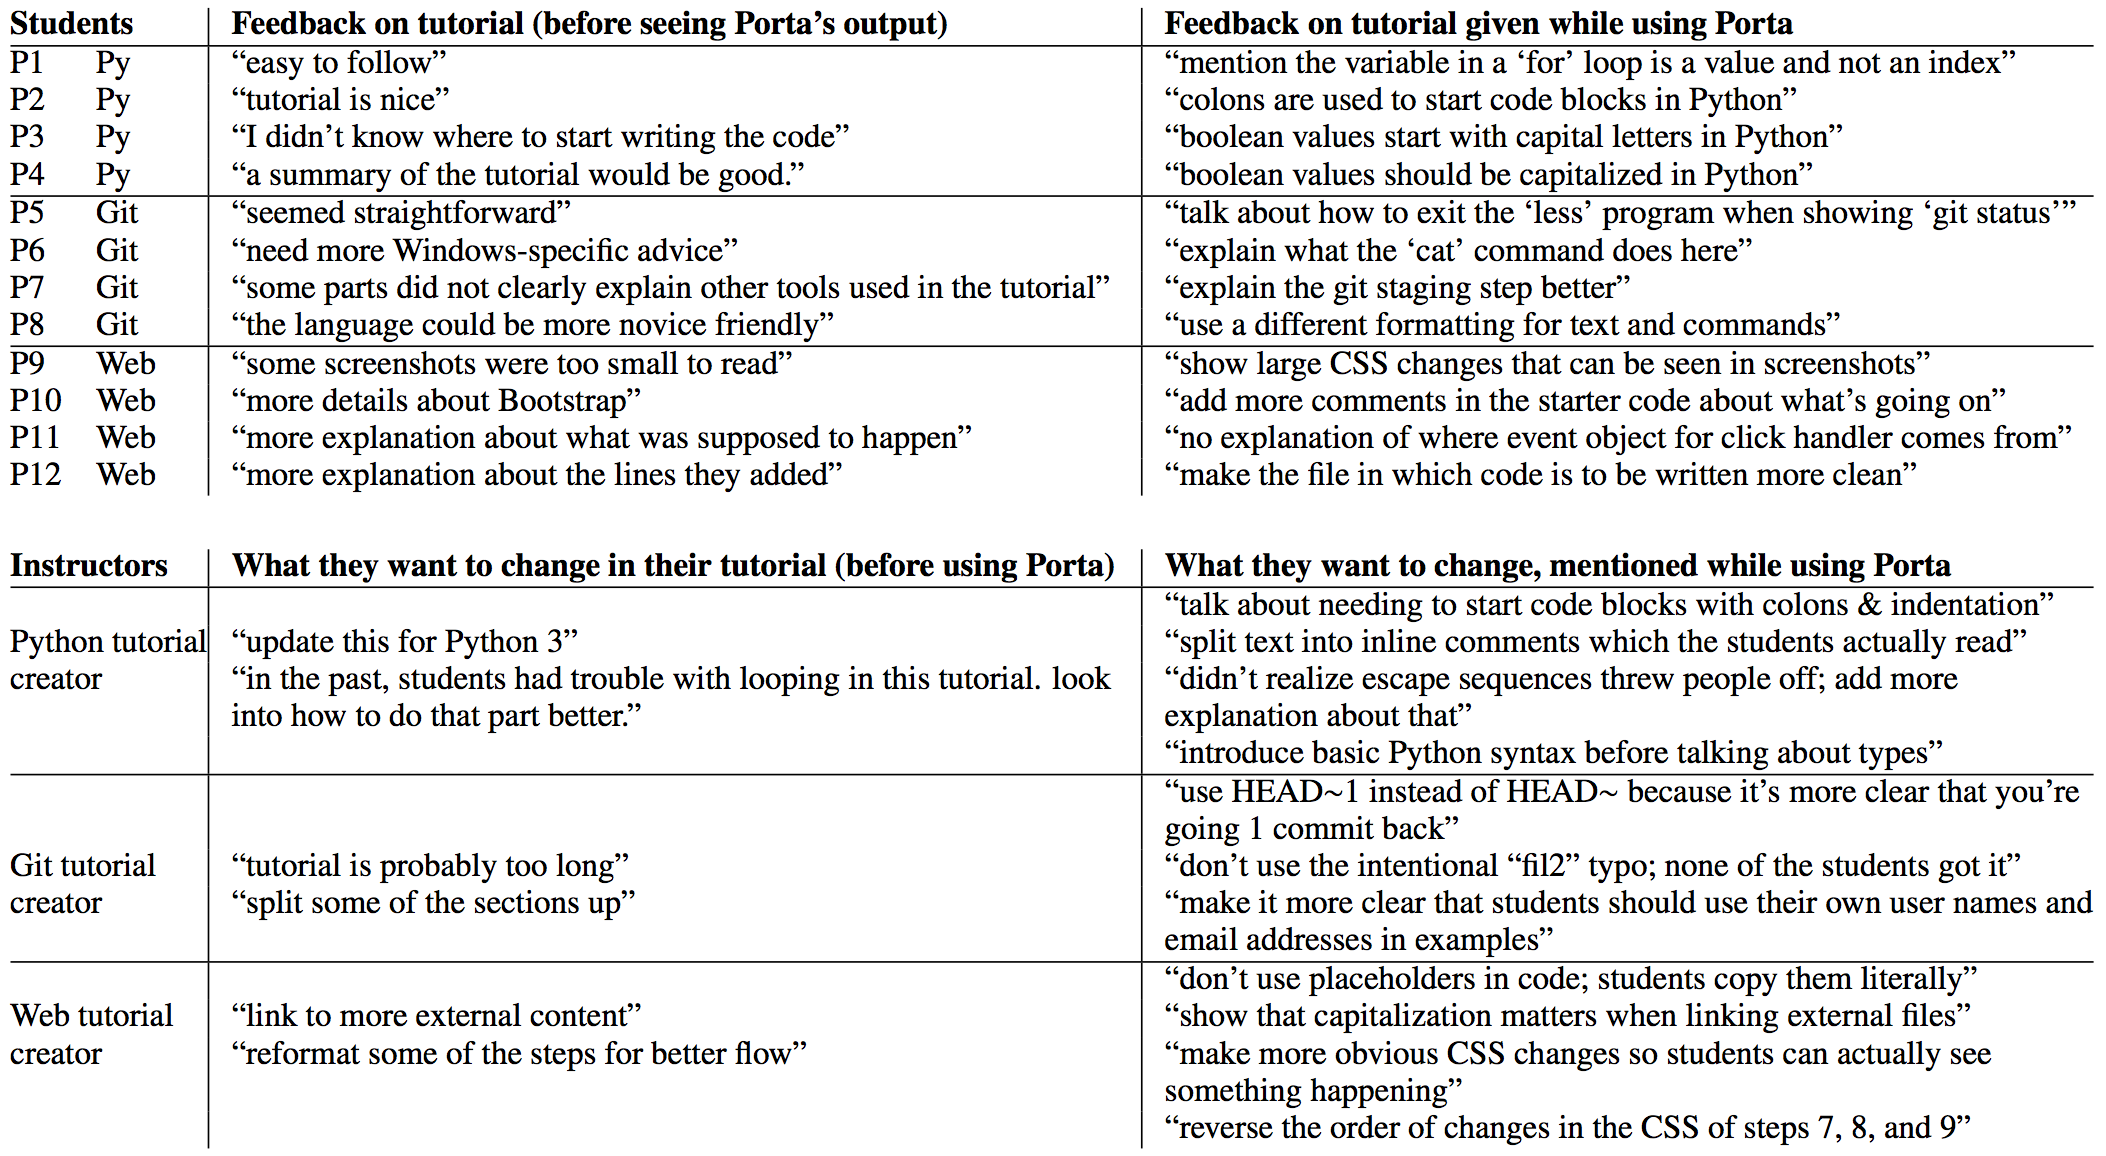
\includegraphics[width=\linewidth]{figures/porta/tbl_feedback.png}
  \caption{Porta uses mouse location as a proxy for where the user's
    attention is focused. a) If the user hovers over anywhere in this code
    block element, Porta will record it as being in focus and b) render it
    as a red hotspot in the sidebar heatmap. c) If the user hovers over an
    element (e.g., background) that is larger than the viewport, that event
    is ignored.}
\end{table}



% Put this info in the table itself:
%
%Abhik said the tutorial should have explained the loop
%variable in a for loop in the value and not an index like Java. Both
%Alexis and Abhik wanted better explanation of using colons and
%whitespace in Python while both Boyan and Sarah wanted the tutorial to
%mention that boolean values start capitalized in Python. Yuhan and Si
%wanted more explanation about the stage and the git status command
%respectively while Ziwen wanted more obvious HTML formatting for
%commands and Stephanie would have liked more explanation about the cat
%command. Angela wanted larger screenshots and more obvious CSS changes
%while Weiwen said that she was confused about which code files she ought
%to have written code in. Jimmy and Kelsey wanted comments in the starter
%code and explanation about how the event object is passed into the click
%handler in Javascript.


% not sure how to incorporate this paragraph from Alok, even though it's
% good stuff!
%
%Some subjects also blamed shortcomings of the tutorials on themselves.
%Both Boyan and Sarah made mistakes with the capitalization of the first
%letter of True and False in Python and blamed it on their previous
%experience with Java even though the tutorial did not make an effort to
%call that out. Abhik said he was not used to whitespaces in Python when
%he made mistakes with indentation even though the tutorial had not
%talked about whitespaces. Stephanie and Si both blamed their inability
%to quit less on the output of git status to not being familiar with the
%unix command line even though the tutorial did not mention how to exit
%less until later.Angela made a mistake typing out CSS color codes and
%when asked about it, she said that the mistake was because she did not
%know the color code syntax even though it was not introduced in the
%tutorial. Kelsey and Weiwen both blamed themselves for not knowing which
%file to type code in when they used the web programming tutorial even
%though the tutorial itself was vague about it.

\begin{comment}

From Alok:

Table 1 summarizes the quantitative data gathered from the consumer user
study. Before the consumers saw their own usage profile, their feedback
for improving the tutorial were either vague or non-existent. 8 out of
the 12 users (Alexis, Sarah, Abhik, Angela, Kelsey, Boyan, Si) thought
that the tutorials they saw were good enough in their current state.
Abhik said the python tutorial was “Easy to follow”. Alexis said about
the python tutorial - she “Liked the tutorial”. Boyan said the Python
tutorial was “nice”. Si thought the git tutorial was “straightforward”.
Angela And Kelsey thought the web development tutorial was “easy to
follow”.

The feedback from the participants we did receive was often vague. Ziwen
thought that the git tutorial “only gave her a basic idea” and that “the
language could be more novice friendly”. Stephanie wanted more Windows
specific advice in the git tutorial since she was a windows user. Jimmy
thought that the web design tutorial “needed more details about
bootstrap”. Weiwen thought that the web programming tutorial needed
“More explanation about what they did”.

Some subjects also blamed shortcomings of the tutorials on themselves.
Both Boyan and Sarah made mistakes with the capitalization of the first
letter of True and False in Python and blamed it on their previous
experience with Java even though the tutorial did not make an effort to
call that out. Abhik said he was not used to whitespaces in Python when
he made mistakes with indentation even though the tutorial had not
talked about whitespaces. Stephanie and Si both blamed their inability
to quit less on the output of git status to not being familiar with the
unix command line even though the tutorial did not mention how to exit
less until later.Angela made a mistake typing out CSS color codes and
when asked about it, she said that the mistake was because she did not
know the color code syntax even though it was not introduced in the
tutorial. Kelsey and Weiwen both blamed themselves for not knowing which
file to type code in when they used the web programming tutorial even
though the tutorial itself was vague about it.

We saw that the feedback we got from the subjects were more actionable
and specific when we guided them through their own data through the
Porta viewer. Abhik said the tutorial should have explained the loop
variable in a for loop in the value and not an index like Java. Both
Alexis and Abhik wanted better explanation of using colons and
whitespace in Python while both Boyan and Sarah wanted the tutorial to
mention that boolean values start capitalized in Python. Yuhan and Si
wanted more explanation about the stage and the git status command
respectively while Ziwen wanted more obvious HTML formatting for
commands and Stephanie would have liked more explanation about the cat
command. Angela wanted larger screenshots and more obvious CSS changes
while Weiwen said that she was confused about which code files she ought
to have written code in. Jimmy and Kelsey wanted comments in the starter
code and explanation about how the event object is passed into the click
handler in Javascript.

\end{comment}


\subsection{Findings from Instructor User Study}

The ultimate goal of Porta is to give useful feedback to tutorial
creators. To assess how well it achieves this goal, we showed the
instructor who created each tutorial the Porta outputs from all 4 of its
student user study sessions. (To evaluate Porta in isolation, we did
\emph{not} show instructors the actual feedback that students provided;
they saw only Porta's outputs.)

% https://docs.google.com/document/d/17KqB676cibTDfvQnhSn0edS5xOe3OXkS3D4TIj8JsRc/edit#

To get baseline impressions, before introducing Porta we asked each
instructor to look over their tutorial and let us know if they wanted to
make any specific changes to it. As the lower left of
\tab{tab:study-feedback} shows, they provided only vague ideas such as
``split some of the sections up." All three felt their tutorial was in
good shape since it had been used by many past students: The Python
tutorial had been used in two iterations of a 400-student data science
course; the Web Design one was used in four iterations of a 300-student
HCI course; and the Git tutorial was featured in a 10,000-student
MOOC. Thus, these instructors had already fixed many issues
from having these tutorials so heavily used over the past few years.

% From Sean Re: Git tutorial "~9800 folks are enrolled in the class on
% Coursera. About 200 people sign up every week. ~1500 users for the
% book every month, 80% of those are unique. 10% of page views are for
% the Git and GitHub part."

\textbf{Expert blind spot effect}: While exploring Porta's
visualizations, all three instructors noticed unexpected student
behavior that surprised them, even despite having taught multiple times
using these instructional materials.
%
This could be an instance of the expert blind spot~\cite{Nathan2001}
whereby experts have trouble relating to what novices know and do not
know since, as experts, they are too familiar with their own subject
matter.

% Despite having taught hundreds of students in multiple courses using
% these tutorial materials, they were still surprised at some of the ways
% in which students struggled. 

All three explored Porta's positional heatmaps to see where students spent
relatively more time and clicked on event markers to see what students
were doing at those locations along with what errors they encountered.
%
For instance, the Python tutorial's creator did not realize that Python
syntax to demarcate code blocks with colon and whitespace was a major
leap for novices. He only realized this when he saw several students
struggling with indentation errors and repeatedly having those error
events show up in Porta's output. The Git tutorial's creator had
mastered Unix command-line tools, so he did not anticipate that students
would have such a hard time using basic commands like `less' and `cat'. The
Web Design tutorial's creator was surprised that students copy-pasted
code with placeholders without filling them in with their own values; to
him, it seemed obvious that, say, the value of the HTML `href' attr
could not literally be the ``..." characters.


%    - user study insight from sean (instructor): "He did not realize
%      that students skipped through a lot of text. The instructions
%      about how to quit `less' when you ran `git status' was there and
%      students spent time trying to exit `less' since they didn't read
%      that part of the text -- needs to make it more clear."


\textbf{Ideas for improving tutorials}: Instructors were also
able to use Porta to come up with actionable ideas for improving their
tutorials. The lower right of \tab{tab:study-feedback} summarizes their
ideas.

For instance, the Python tutorial's creator saw from heatmap
visualizations that most students did not even read through major parts
of his tutorial. He realized that reformatting those parts as inline
comments in code examples might work better. Also, from observing the
temporal order of events, he came to the conclusion that he should have
introduced code blocks and whitespace significance in the tutorial first
before introducing Python types.
%
The Git tutorial's creator was surprised that adding in an intentional
typo for ``fil2" tripped up all the students who encountered it. He
expected students to run the command verbatim with the typo, but
everyone actually used the correct spelling of ``file2" and therefore
got confused by the next section that explained the consequences of the
intentional mistake. He now plans to remove this section.
%
The Web Design tutorial's creator concluded that he should have made CSS
style changes more obviously salient. In the current tutorial, the
visual changes were too subtle to notice.

% good stuff, but too long for now:
%During an end-of-session debriefing, all three instructors mentioned
%that if Porta were used to regularly test tutorials, it would serve as a
%forcing function for them to continuously improve their tutorials. The

%All three instructors wanted to use Porta. The Python tutorial's creator
%said, ``you're very rarely sitting down with students when building
%tutorials, so feedback is lacking." The Git tutorial's creator said that
%``the perennial problem is motivating MOOC creators to update their
%content because they don't know what to change. Going back and fixing
%things is painful without direct feedback. Porta could help with that."

%and that they ``rarely re-evaluated the value of existing tutorials."

%Finally, the Web Design tutorial's creator noted that ``students very
%rarely ever give feedback about the state of existing materials" except
%when there are obvious bugs.

In theory, instructors could have gleaned these insights via direct
observation or by watching videos of test sessions. However, needing to
directly observe users limits scale, whereas Porta could be used to run
user tests remotely and be administered by third parties. It would also
likely take them much longer to watch the raw videos, and they would not
get the benefits of Porta's heatmaps or event markers to hone in on
clusters of related user activities. Finally, Porta provides a compact
summary of test sessions that can easily be shared with other people
such as co-instructors or future students.

\begin{mynote}

\textbf{Summary}: Porta allowed tutorial creators to discover surprising
insights about student behavior and also come up with specific
actionable ideas for improving their tutorials.

\end{mynote}
